\documentclass{article}

\usepackage{PRIMEarxiv}
\usepackage[utf8]{inputenc}
\usepackage[T1]{fontenc}
\usepackage{hyperref}
\usepackage{url}
\usepackage{booktabs}
\usepackage{amsmath}
\usepackage{amsfonts}
\usepackage{microtype}
\usepackage{graphicx}
% preamble
\usepackage{tikz}
\usetikzlibrary{arrows.meta, positioning}
\title{Extending Neural Networks: Lateral Propagation and Multimodal Convolution}

\author{
	Jay Kumar \\
	Independent Researcher \\
	Austin, TX \\
	\texttt{j.kumar.nbl@gmail.com}
}

\begin{document}
	
	\maketitle
	
	\begin{abstract}
		Neural network architectures have traditionally evolved along two largely independent axes: improvements in learning mechanisms and improvements in representational capacity. Recurrent neural networks rely on backpropagation through time (BPTT) to model temporal dependencies, while convolutional neural networks (CNNs) exploit spatial locality and are primarily applied to visual domains.
		
		In this work, we decouple these dimensions and investigate two orthogonal extensions. First, we introduce a persistent-memory sequence model that replaces BPTT with localized updates and lateral propagation. Second, we demonstrate that convolution can be extended beyond visual domains to multimodal structured data.
		
		Experimental results show that localized propagation produces stable training behavior with low computational overhead, while multimodal convolution improves generalization as data scale increases. Although limitations remain, particularly in generalization for the local propagation model, these results suggest that neural architectures can be redesigned at a higher level of abstraction by independently modifying learning and representation mechanisms.
	\end{abstract}
	
	\keywords{Recurrent Neural Networks \and Convolutional Neural Networks \and Lateral Propagation \and Multimodal Learning \and Persistent Memory}
	
	\section{Introduction}
	
	Recurrent neural networks (RNNs) and convolutional neural networks (CNNs) represent two foundational paradigms in modern machine learning \cite{goodfellow2016deep, lecun1998gradient}. Despite their success, both architectures are constrained by specific design assumptions.
	
	RNNs rely on backpropagation through time (BPTT), which introduces significant computational overhead and limits scalability. CNNs, while highly effective, are typically treated as domain-specific architectures for visual data.
	
	In this work, we argue that these architectures can be understood at a higher level of abstraction. Specifically, we treat:
	
	\begin{itemize}
		\item Learning mechanisms (e.g., backpropagation vs localized updates)
		\item Representation strategies (e.g., unimodal vs multimodal convolution)
	\end{itemize}
	
	as independent design dimensions.
	
	We explore two corresponding extensions:
	
	\begin{enumerate}
		\item A persistent-memory sequence model that replaces BPTT with localized lateral propagation
		\item A multimodal convolutional framework that generalizes CNNs beyond visual domains
	\end{enumerate}
	
	Together, these contributions suggest that neural architectures can be extended by decoupling learning dynamics from representational structure.
	
	\section{Background}
	
	Traditional RNNs propagate information through hidden states and optimize parameters via gradient descent across time steps. While effective, this approach suffers from vanishing gradients and high computational cost.
	
	Early neural models such as the perceptron \cite{rosenblatt1958perceptron} and connectionist frameworks \cite{rumelhart1986pdp} established the basis for distributed learning. Hebbian learning \cite{hebb1949organization} further motivates localized update rules.
	
	CNNs address structured learning by exploiting locality through shared weights and hierarchical feature extraction \cite{lecun1998gradient}. However, their application has remained largely restricted to visual data.
	
	Recent architectures such as transformers aim to address these limitations but often introduce substantial computational overhead.
	
	\section{Methodology}
	
	\subsection{Persistent-Memory Sequence Model}
	
	We propose a sequence learning model that replaces BPTT with localized updates using persistent memory structures.
	
	The model consists of:
	
	\begin{itemize}
		\item \textbf{Node Memory}: Stores token-position relationships conditioned on class labels
		\item \textbf{Lateral Memory}: Stores token-to-token transitions
		\item \textbf{Class Statistics}: Tracks class frequency for normalization
	\end{itemize}
	
	Training occurs through incremental updates to these structures. During inference, class scores are computed as:
	
	\begin{equation}
		S(c) = \alpha \cdot M_{pos}(c) + \beta \cdot M_{lat}(c) + \gamma \cdot F(c)
	\end{equation}
	
	where:
	\begin{itemize}
		\item $M_{pos}$ represents positional matches
		\item $M_{lat}$ represents lateral transitions
		\item $F(c)$ is the class frequency normalization
	\end{itemize}
	
	This formulation replaces global gradient propagation with localized accumulation and inference.
	
	\subsection{Multimodal Convolution}
	
	We extend convolutional architectures to multimodal structured data.
	
	Each modality (e.g., visual frames, audio spectrograms) is processed through an independent convolutional pathway. These representations are then fused at a higher level.
	
	This approach reframes convolution as a general mechanism for learning localized structure rather than a vision-specific technique.
	\section{Experimental Setup}

Experiments were conducted using the Human Activity Recognition Video Dataset from Kaggle, consisting of labeled video samples across multiple activity classes. The dataset contains approximately 15 GB of video data organized into class-specific directories.

Videos were split into training and testing sets using an 80/20 split. To evaluate the effect of data scale, training subsets of size 500, 1000, and 1500 were requested. However, the effective training size was bounded by the available data after splitting, resulting in a maximum usable training size of 890 samples.

The reduction in effective training size is due to class-balanced sampling and dataset partitioning constraints.

Each video was processed into two modalities:

\begin{itemize}
	\item \textbf{Visual modality}: Each video was uniformly sampled into $T = 8$ RGB frames, resized to $128 \times 128$, and normalized to $[0,1]$.
	\item \textbf{Audio modality}: Audio was extracted at 16 kHz for a duration of 4 seconds and converted into a log-spectrogram of size $128 \times 128$.
\end{itemize}

The multimodal CNN was trained using the Adam optimizer with a learning rate of $10^{-3}$ and weight decay of $10^{-4}$. Models were trained for 5 epochs with a batch size of 8. Cross-entropy loss was used for optimization.

All experiments were implemented in PyTorch. Performance was evaluated using classification accuracy on held-out test data.

	\subsection{Multimodal CNN Architecture}

The multimodal convolutional model processes each video sample as two synchronized modalities: visual frames and audio. For the visual modality, each video is uniformly sampled into $T$ RGB frames, resized to $128 \times 128$, and normalized to $[0,1]$. Each frame is passed through a convolutional branch consisting of four convolutional blocks with batch normalization, ReLU activations, pooling, and adaptive average pooling. The resulting per-frame embeddings are averaged across time to produce a single visual representation.

For the audio modality, the audio stream is extracted at 16 kHz, converted into a log-spectrogram, resized to $128 \times 128$, and passed through an independent convolutional branch. This branch produces an audio embedding of the same dimensionality as the visual embedding.

The two modality embeddings are concatenated and passed through a fully connected classifier:

\begin{equation}
	z_v = f_v(X_v), \qquad z_a = f_a(X_a)
\end{equation}

\begin{equation}
	z = [z_v ; z_a]
\end{equation}

\begin{equation}
	\hat{y} = \mathrm{softmax}(g(z))
\end{equation}

where $X_v$ denotes the sampled video frames, $X_a$ denotes the audio spectrogram, $f_v$ and $f_a$ are the visual and audio convolutional branches, and $g$ is the final multilayer classifier.
\begin{figure}[t]
	\centering
	\resizebox{\linewidth}{!}{
		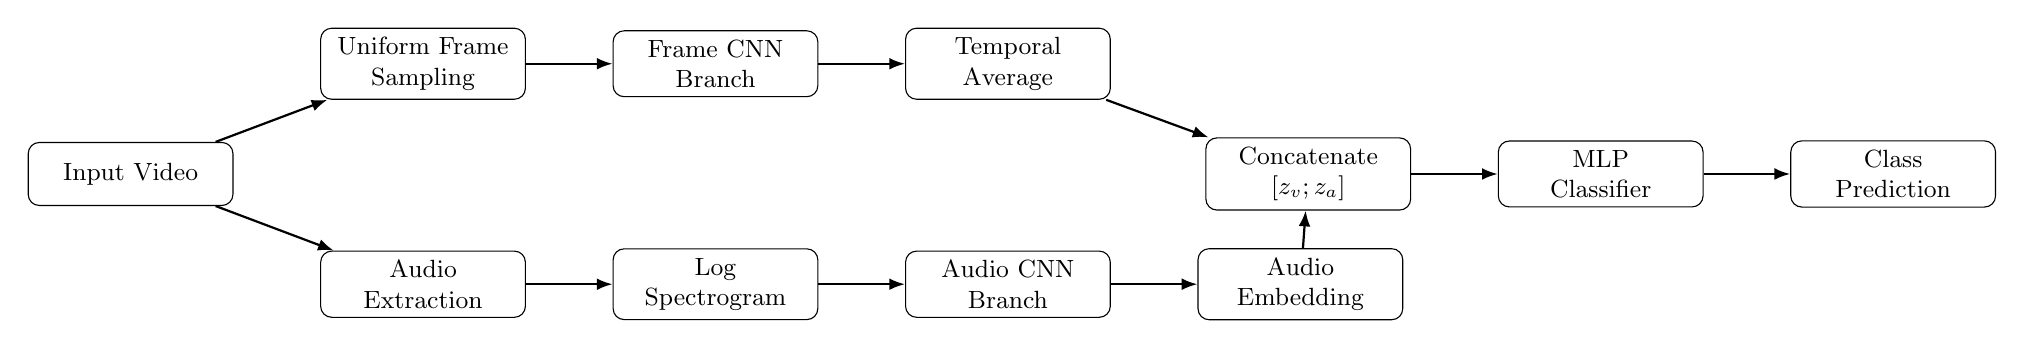
\begin{tikzpicture}[
			node distance=0.9cm and 1.1cm,
			block/.style={
				draw,
				rounded corners,
				align=center,
				minimum width=2.6cm,
				minimum height=0.8cm,
				font=\small
			},
			arrow/.style={-{Latex[length=2mm]}, thick}
			]
			
			\node[block] (video) {Input Video};
			
			\node[block, right=of video, yshift=1.4cm] (frames)
			{Uniform Frame\\Sampling};
			
			\node[block, right=of frames] (framecnn)
			{Frame CNN\\Branch};
			
			\node[block, right=of framecnn] (frameavg)
			{Temporal\\Average};
			
			\node[block, right=of video, yshift=-1.4cm] (audio)
			{Audio\\Extraction};
			
			\node[block, right=of audio] (spec)
			{Log\\Spectrogram};
			
			\node[block, right=of spec] (audiocnn)
			{Audio CNN\\Branch};
			
			\node[block, right=of audiocnn] (audioemb)
			{Audio\\Embedding};
			
			\node[block, right=1.2cm of frameavg, yshift=-1.4cm] (concat)
			{Concatenate\\$[z_v;z_a]$};
			
			\node[block, right=of concat] (mlp)
			{MLP\\Classifier};
			
			\node[block, right=of mlp] (pred)
			{Class\\Prediction};
			
			\draw[arrow] (video) -- (frames);
			\draw[arrow] (frames) -- (framecnn);
			\draw[arrow] (framecnn) -- (frameavg);
			\draw[arrow] (frameavg) -- (concat);
			
			\draw[arrow] (video) -- (audio);
			\draw[arrow] (audio) -- (spec);
			\draw[arrow] (spec) -- (audiocnn);
			\draw[arrow] (audiocnn) -- (audioemb);
			\draw[arrow] (audioemb) -- (concat);
			
			\draw[arrow] (concat) -- (mlp);
			\draw[arrow] (mlp) -- (pred);
			
		\end{tikzpicture}
	}
	\caption{Multimodal CNN architecture. Each video is represented using sampled RGB frames and an audio-derived log-spectrogram. Independent convolutional branches produce modality-specific embeddings, which are concatenated and classified using a multilayer perceptron.}
	\label{fig:multimodal-cnn}
\end{figure}

The following section evaluates both proposed approaches under the experimental setup described above.
	
	\section{Results}
	
	\subsection{Local Propagation}
	
The persistent-memory model achieves stable training behavior across all evaluated training sizes. Training accuracy remains consistent, indicating that the model successfully captures structure within the training data.

However, generalization fails entirely under the current formulation, with test accuracy collapsing to zero across all configurations. This indicates that while localized propagation captures training structure, it does not produce transferable representations for unseen data.
	

	
	\begin{table}[h]
		\centering
		\begin{tabular}{lccc}
			\toprule
			Metric & 500 & 1000 & 1500 \\
			\midrule
			Train Accuracy & 0.668 & 0.670 & 0.646 \\
			Test Accuracy & 0.000 & 0.000 & 0.000 \\
			\bottomrule
		\end{tabular}
		\caption{Persistent-memory model performance}
	\end{table}
	
	These results indicate that while localized propagation captures structure during training, it lacks mechanisms for robust generalization.
	
	\subsection{Multimodal Convolution}
	
The multimodal CNN demonstrates a clear improvement in generalization as training data increases. Test accuracy improves from 41.3\% to 63.7\% as the training set grows, while training accuracy increases only modestly.

This pattern suggests that additional data primarily improves generalization rather than memorization.
	
	\begin{table}[h]
		\centering
		\begin{tabular}{lcc}
			\toprule
			Metric & 500 Samples & 890 Samples \\
			\midrule
			Train Accuracy & 0.500 & 0.556 \\
			Test Accuracy & 0.413 & 0.637 \\
			\bottomrule
		\end{tabular}
		\caption{Multimodal CNN performance}
	\end{table}
	
The improvement in test accuracy suggests that convolution operates over structured relationships rather than modality-specific features, supporting the hypothesis that convolution is a general mechanism for learning local structure.
	
	Notably, average prediction confidence remains relatively stable across runs, suggesting that improvements in accuracy are driven by more correct predictions rather than increased model certainty.
	\section{Discussion}
	
	\subsection{Learning Without BPTT}
	
	The persistent-memory model demonstrates that sequence learning can occur without global temporal gradient propagation. However, the lack of generalization indicates the need for additional mechanisms, such as global constraints or normalization.
	
	\subsection{Generalizing Convolution}
	
	The multimodal results support the hypothesis that convolution is not inherently tied to visual data, but to structured locality.
	
	\subsection{Abstraction as a Design Principle}
	
	These findings suggest that neural architectures can be extended along independent axes of learning and representation, enabling more flexible system design.
	
	\subsection{Limitations}
	
	The proposed approaches exhibit several limitations. The persistent-memory sequence model fails to generalize beyond training data, indicating that local propagation alone is insufficient for robust sequence learning.
	
	The multimodal CNN, while effective, relies on relatively simple fusion via feature concatenation. More sophisticated fusion mechanisms may better capture cross-modal interactions.
	
	Additionally, experiments were conducted on a single dataset, and further validation across diverse domains is required.
	
	\section{Conclusion}
	
	We presented two extensions to neural network design: localized lateral propagation for sequence learning and multimodal convolution for structured representation.
	
	While limitations remain, these results demonstrate that neural networks can be restructured at a higher level of abstraction, decoupling learning mechanisms from representation strategies.
	
	Future work will focus on improving generalization in localized propagation models and refining multimodal fusion techniques.
	
	\bibliographystyle{unsrt}
	\bibliography{references}
	
\end{document}